\subsubsubsection{Interaction between entities}

The application contains several interactions among entities that have to be
specified in order to understand well how to approach different problems.

\paragraph{Entering a road} Moving entities enter a road by accessing a stretch
that is located at the beginning of the road and that is treadable by their
specific entity type.

\paragraph{Entering a road stretch} 
Moving entities who want to enter a new road stretch
can do it whenever there is room for them in that stretch. 
In particular, a roadway lane stretch can be trod for at most 
one vehicle at a time.

\paragraph{Zebra crossings} Vehicles which want to enter a road stretch 
with painted zebra crossings, have to wait for 
pedestrians or bikes to free all stretches of the crossing.

\paragraph{Changing roadway lane} A vehicle that is on the i-th road stretch
which desires to change lane has to wait until the (i+1)-th stretch in the
wanted direction is empty.

\paragraph{Crossroads} Every road that is connected to a crossroads is marked
with a cardinal point (N/E/W/S). The crossroads holds all the logic necessary
for vehicles to follow the yield rules we described in
\ref{sec:pa-domain-problems}.

% verifica risposta Sebastiano
However there could be a situation in which there is a standstill,
for example when four cars simultaneously want to go straight in
a four-way crossroads each one by entering a different way of it.
In this case, the crossroads has to make a car yield the right-of-way to another one.

Pedestrians can only walk on the corner of the crossroads, thus passing to the
adjacent piece of road. For example, a pedestrian that is coming from 
the ``southern'' side of the western road can only enter the southern street 
on the ``western'' side.

\paragraph{Entering a building} When a moving entity is in the stretch where
there is the entrance of a building, then it can enter the building.
If such an entity is a vehicle, it has to wait for all other entities who
are in the intermediate stretches to move away.

\paragraph{Exiting a building} When a moving entity is exiting a building, it
has to check whether there is room for it to move out.
If such an entity is a vehicle, it has to yield the right-of-way to 
upcoming vehicles and to wait for potential sidewalks or bicycle path stretches 
facing the building to be empty too.

\paragraph{Choosing to use a vehicle} A person $p$ who wants to leave a
building $a$ to move to a $b$ one can decide to take an available vehicle.

When $p$ requires to get out it with a vehicle,
all other people in $a$
\begin{itemize}
  \item sharing the same path; or
  \item having a destination $c$ contained into $p$'s path; or
  \item having a path containing $b$
\end{itemize}
can decide to leave $a$ with $p$ sharing a vehicle
until the most capacious vehicle, among the available, ones become full.

Nevertheless $p$ can leave $a$ with a vehicle only if:
\begin{itemize}
  \item the capacity of $b$'s car park is greater than the sum of all 
vehicles being already there and the ones which are coming there; or
  \item there are at least another people in $a$ 
  \begin{itemize}
    \item having a path containing $b$; and
    \item ending with a building $d$, having a car park capacity that is greater than 
	the sum of all vehicles being already there and the ones which are coming there.
  \end{itemize}
\end{itemize}
Hence, if the condition is met, the destination building books a parking lot for the vehicle.

\begin{figure}[H]
  \centering
  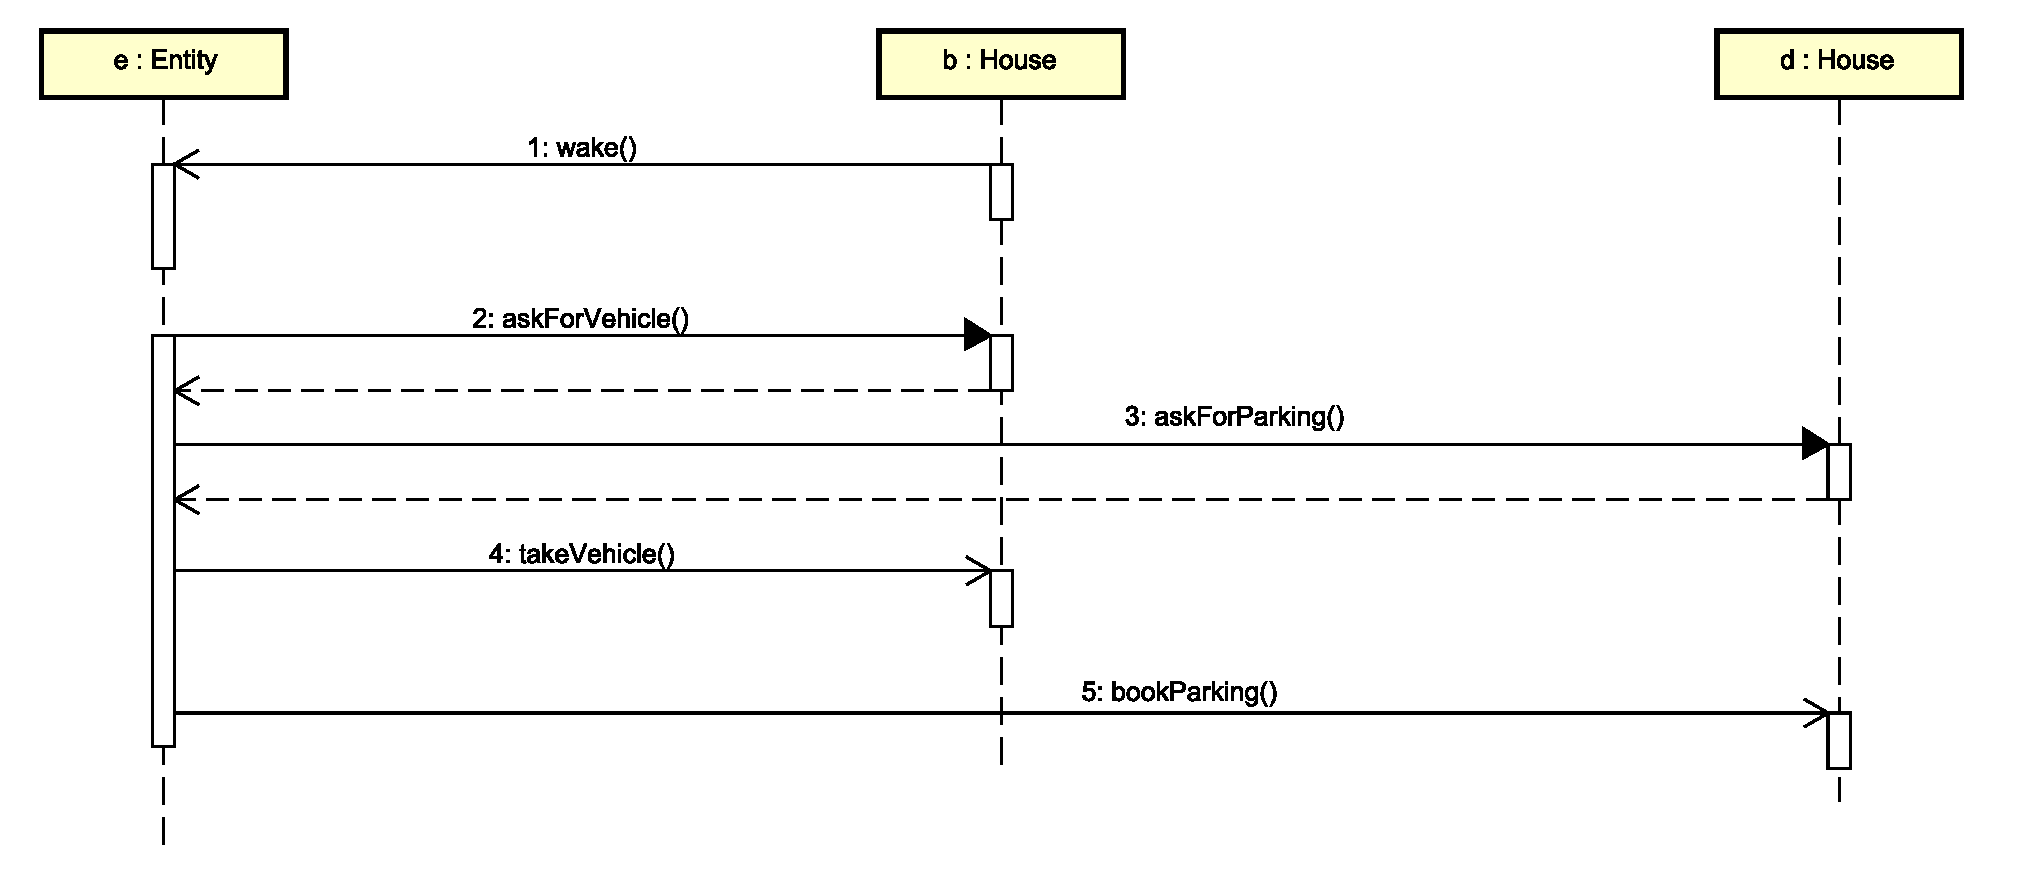
\includegraphics[width=\columnwidth,trim=1 0 0 0,clip]
    {sections/images/solution/going-out-vehicle.eps}
  \caption{Exiting a building with a vehicle}
  \label{fig:app-inter-vehicle}
\end{figure}

\paragraph{Waiting for a bus} 
Whenever a pedestrian is on a bus stop stretch, 
it can decide to wait for a bus.

Firstly, the pedestrian checks whether its path is (even partially) 
matched by the busses one.
If at least one of them does, then it waits for a limited amount of time for a bus to arrive.

If this timeout expires, then it continues travelling by foot to the next stretch.

\begin{figure}[H]
  \centering
  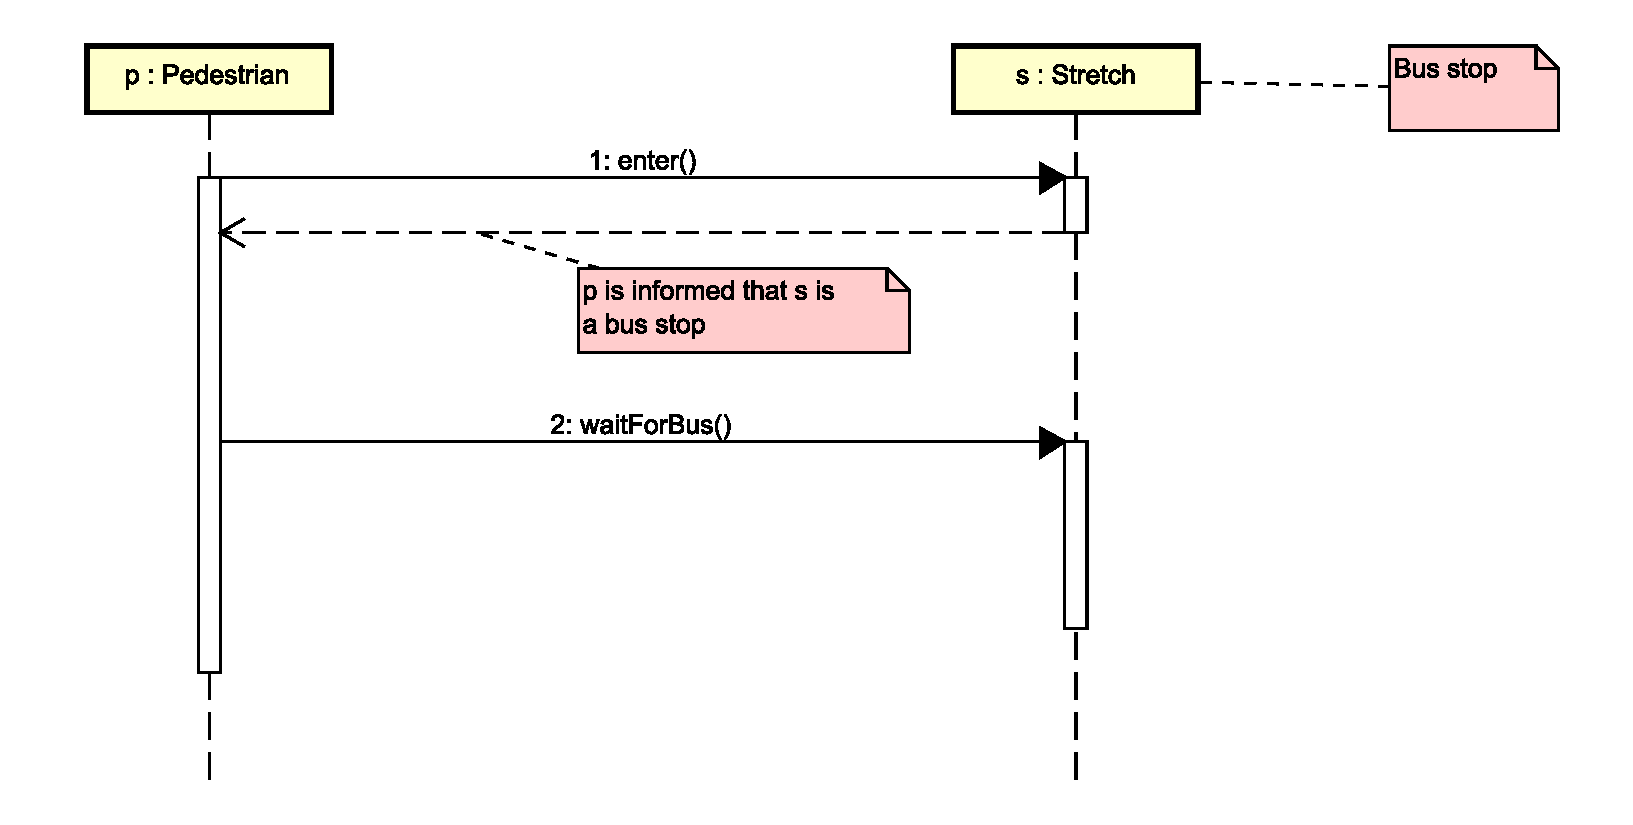
\includegraphics[width=\columnwidth,trim=1 0 2 0,clip]
    {sections/images/solution/bus-waiting.eps}
  \caption{Waiting for a bus}
  \label{fig:app-inter-wait-bus}
\end{figure}

\paragraph{Boarding a bus} When a bus arrives at a bus stop, then a waiting
pedestrian will board it only if:

\begin{itemize}
  \item there is enough room for it; and
  \item this bus shortens the expected route for it.
\end{itemize}

\begin{figure}[H]
  \centering
  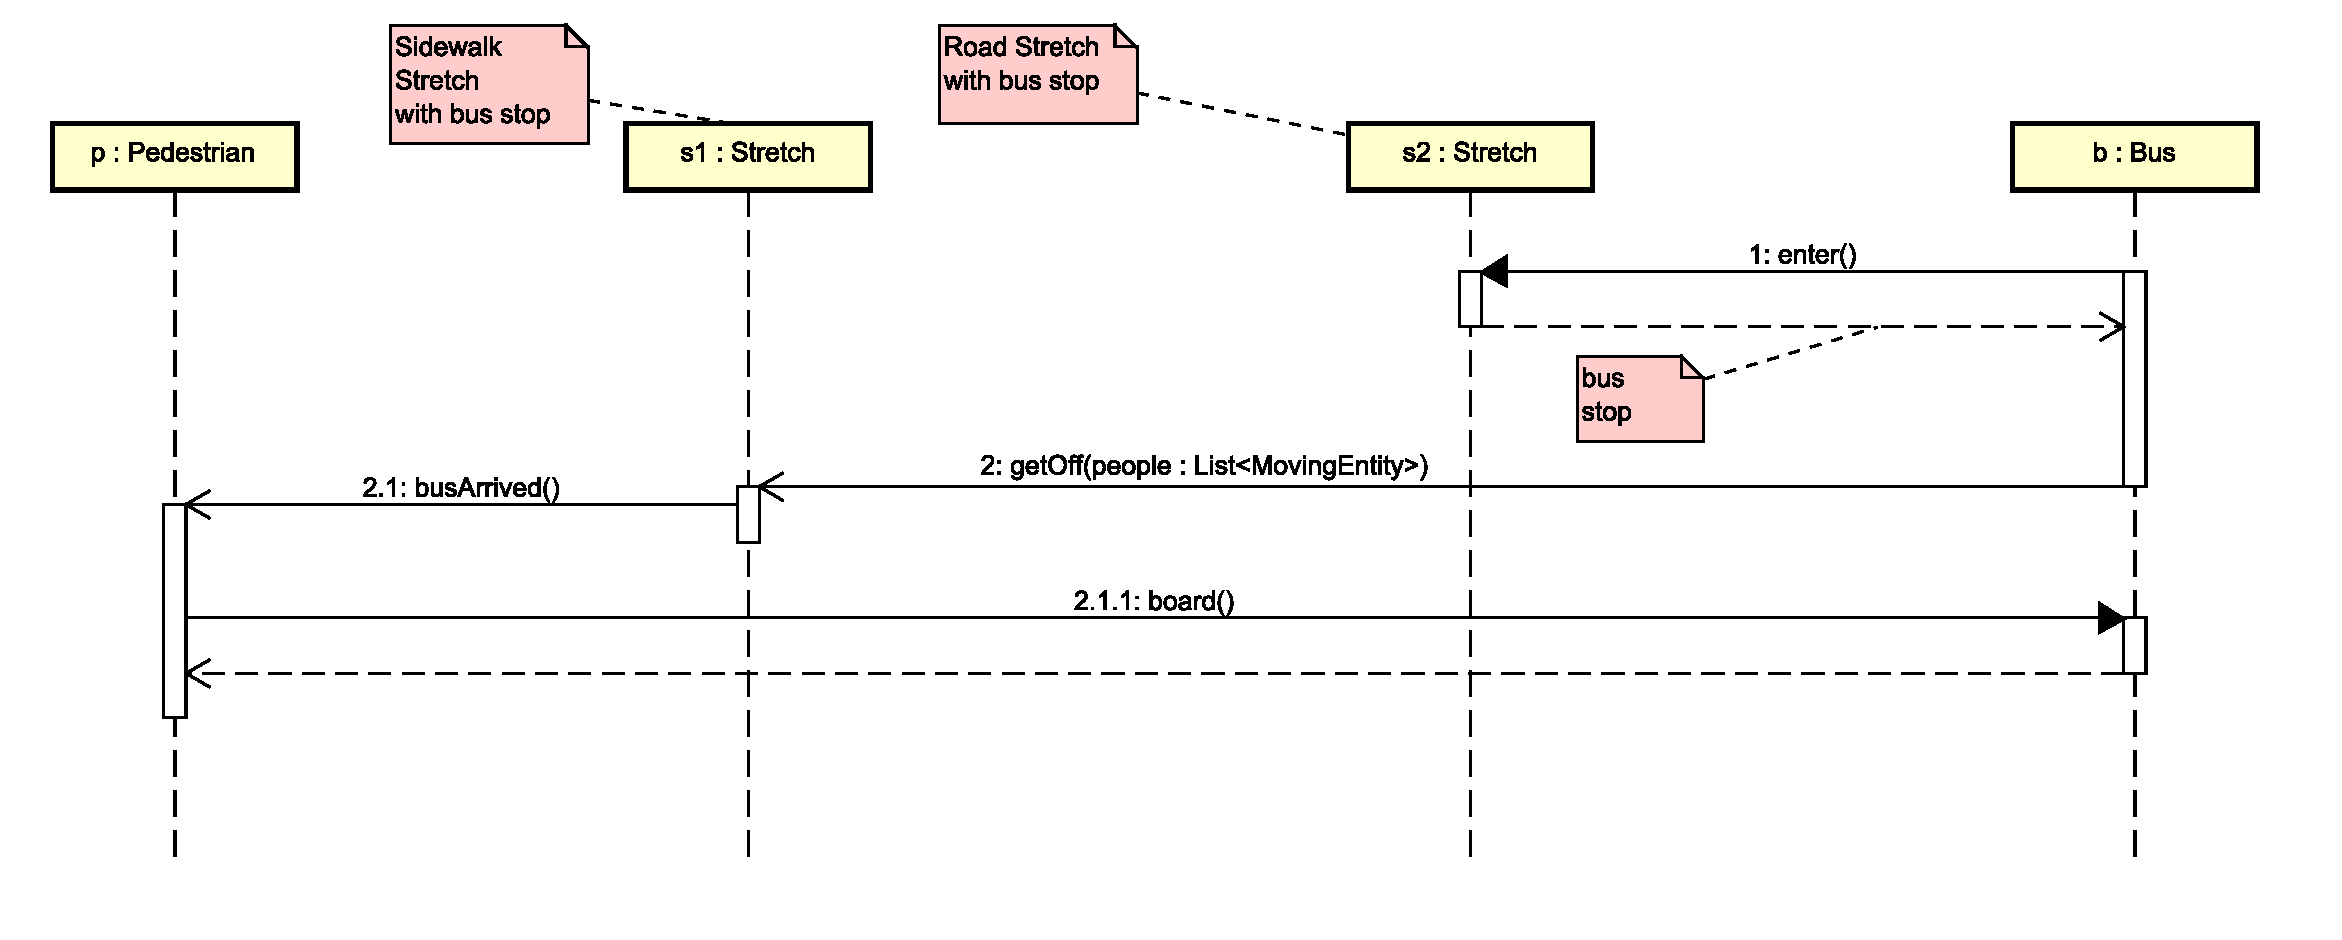
\includegraphics[width=\columnwidth,trim=1 0 0 0,clip]
    {sections/images/solution/bus-boarding.eps}
  \caption{Boarding a bus}
  \label{fig:app-inter-board-bus}
\end{figure}

\paragraph{Getting off a bus} A person $p$ will get off a bus when it reaches
the last stop $s$ belonging to the route of $p$.

\paragraph{Respecting street code} Roads and crossroads have to contain 
all the logic which is needed to make moving entities follow the street rules.

\paragraph{Performing an overtaking} This action is possible only when a
vehicle is able to change lane. It might be triggered by a timeout which
expires when it is waiting too much for entering the next straightaway stretch.

When a vehicle tries to overtake another one, it will always try to return to
the lane where it started the operation before entering the last stretch.
% look for "manovra" translation

% \paragraph{Uber} % Is it a TODO?

